%====================================================================================================
% Possibilities and choices
%====================================================================================================
\section{Possibilities and choices}
\subsection{Possibilities}
\subsubsection{measurement method}
Two options are available for creating the software:
\begin{enumerate}
    \item \textbf{Pre-capture of images using Vimba software (\ref{sec:Vimba})} : \newline
          In this case, the images are taken using the software supplied with the camera and then entered into the software develop with python.
          The problem is that the operator carrying out the measurement will have to switch between initialization parameters and parameters
          for measurements on the Vimba software. For this solution, different software modes will also be required
    \item \textbf{Image capture and analysis} :\newline
          The second solution involves automatic measurement and initialization. The operator would simply point the telescope at an
          object and launch the software. The problem with this solution is that it would be more complex to detect a bug. In this case,
          we'd have to come up with solutions to recognize measurement bugs as quickly as possible.
\end{enumerate}
\subsubsection{Initialization}
For initialization, two solutions are also possible :
\begin{enumerate}
    \item The first is to take several images with a exposure time equal to the measurement part. By adding up all the images,
          the turbulence will be averaged. It will then be easy to determine the object's center of gravity and its centroid.
    \item The second option would be to considerably increase the exposure time of the image. This would be the same as the
          previous option, but taking only 1 image would reduce memory usage and increase computing speed.
\end{enumerate}
In these 2 cases, the number of images to be used or the exposure time required to correctly average the image will need to
be determined during the initial tests. If turbulence is not properly averaged, aberrant results may appear.
\subsection{Choices}
\subsubsection{measurement method}
The software will feature both methods of use. However, the pre-capture method with Vimba software will not yet be implemented in its first version.
The addition of this possibility could be agreed at a later date if there is a real interest.
\subsubsection{Initialization}
The chosen initialization method is to take several images with minimal pause time. \newline
Using a longer pause time could result in unwanted elements appearing in the image.
What's more, the images used during initialization could be reused for measurement. The basic principle of initialization is :
\begin{itemize}
    \item Take \textit{X} images to average turbulence.
    \item Recognition of centers of interest.
    \item Localization of image centers.
    \item Recovering the size of the centers of interest for cropping during measurement.
\end{itemize}
The number of images to be taken for the centroid to be as accurate as possible will be determined during testing.
If the disturbance is measured on a star, it is possible to take images in an automated way until the average image
is as circular as possible (the star would have been deviated at any point internal to the turbulence).
\subsubsection{Measurement}
The measurement program will be simple in principle. However, when image processing is involved in a process, the main issue is reliability.
The measurement program must :
\begin{itemize}
    \item Take a shot with the shortest possible exposure time.
    \item Image adjustment.
    \item Find the 2 points of interest in the image.
    \item Determine their centroid.
    \item Recover the result of the difference with the initialization centroid.
    \item Repeat the above points several times.
    \item Calculate the variance of centroid deviations
    \item Transform value into Fried parameter
\end{itemize}
As stated at the beginning of this section, image processing is a very sensitive element in the program. To achieve this,
multiple tests will have to be carried out in order to certify the robustness of its use.
%====================================================================================================
% Vimba software
%====================================================================================================
\newpage
\section{Vimba software}\label{sec:Vimba}
The Vimba software package was created by Allied Vision and is available to all users of Allied Vision cameras.
The software lets you modify camera parameters in real time (Figure \ref{fig:Soft_Vimba}). It is also designed to pre-process
the image before sending it for output. Inputs are also available to control the camera.
\begin{figure}[H]
    \centering
    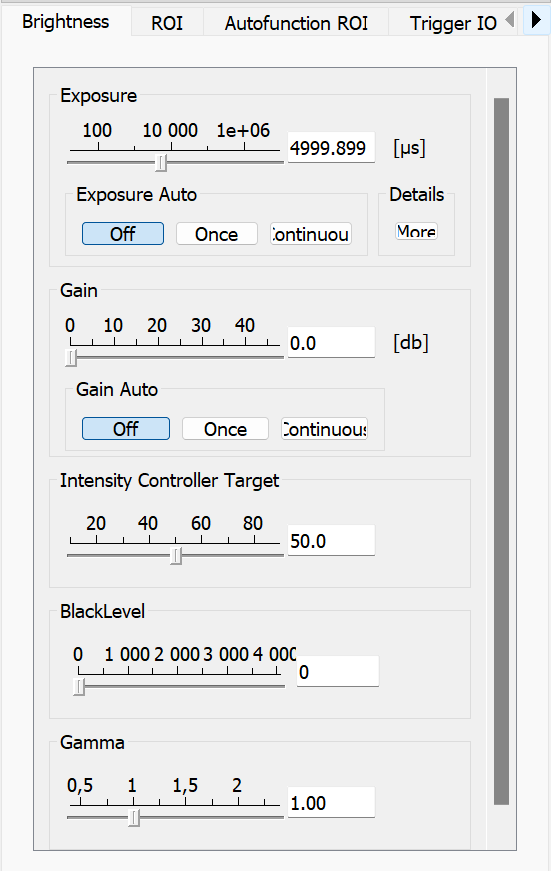
\includegraphics[scale=0.85]{assets/figures/Software/VimbaInterface.png}
    \caption{Editable image parameters on Vimba}
    \label{fig:Soft_Vimba}
\end{figure}
This application is very useful for adjusting parameters during measurements, but also for initial tests, as several images can
be taken in quick succession using one of the software's functions (With the "Image series options" parameter).
%====================================================================================================
% Python API for Vimba
%====================================================================================================
\newpage
\section{Python API for Vimba}
The Vimba software introduced in section \ref{sec:Vimba} is also supplied with an API for simulating the software on python.
All API data is given in a git directory (\href{https://github.com/alliedvision/VimbaPython}{Github link}) and the user manual
can be found in appendix \ref{App:pythonVimba}.\newline
Please note that if the Vimba program is open on the computer, the API will not be able to communicate with the camera.
\subsection{Camera connection}\label{sec:Soft_API_Connect}
Before using the camera with the API, the code must call the procedure that simulates the Vimba program :
\begin{verbatim}
    with Vimba.get_instance() as vimba:
        cams = vimba.get_all_cameras()
        with cams[0] as cam:
            // Your code
\end{verbatim}
In the code above, the "cam" structure is the element to be called in order to access all the camera parameters.
With this structure, image parameters, setups and access to images can be carried out.
\subsection{Parameter modification}
The API also lets you change camera parameters separately. In the case of the \Gls{DIMM} application, the most important
need is to change the exposure time. To do this, once the camera is connected (Code in section \ref{sec:Soft_API_Connect}),
call this function:
\begin{verbatim}
    exposure_time.set(2000) #us
\end{verbatim}
This function lets you change the exposure time (given in microseconds) and can range from 20 to 10000000 (10 seconds).
\subsection{Load and save settings}
\subsubsection{Save settings}
Pre-recorded settings files can be created for the camera. If certain values are modified and you wish to keep them,
you can save the file on your computer. To do this, after connecting to the camera (\ref{sec:Soft_API_Connect}),
simply call up the function :
\begin{verbatim}
    settings_file = 'my_File.xml'
    cam.save_settings(settings_file, PersistType.All)
\end{verbatim}
\subsubsection{Load settings}
To retrieve settings that have already been saved and load them into the camera, use the code below:
\begin{verbatim}
    settings_file = 'my_File.xml'
    cam.load_settings(settings_file, PersistType.All)
\end{verbatim}
\newpage
\subsection{Image capture}
Before taking an image, you need to be able to set a format compatible with the compiler or
a library that will be used to create the software. To do this, the following code compares
the camera's available formats with the compatible formats.
\begin{verbatim}
    with Vimba.get_instance() as vimba:
        cams = vimba.get_all_cameras()
        with cams[0] as cam:
            formats = cam.get_pixel_formats()
            opencv_formats = intersect_pixel_formats(formats, OPENCV_PIXEL_FORMATS)
        print(f"Available formats:")
        for i, format in enumerate(formats):
            print(i, format)
        print(f"\nOpencv compatible formats:")
        for i, format in enumerate(opencv_formats):
            print(i, format)
\end{verbatim}
\begin{figure}[H]
    \centering
    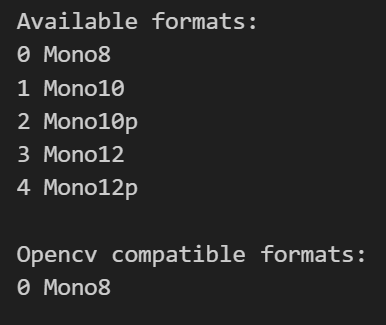
\includegraphics[scale=0.85]{assets/figures/Software/Format_Available.png}
    \caption{Compatible format results}
    \label{fig:Soft_Vimba_Format}
\end{figure}
Once the correct parameters have been displayed, simply call up this line of code, inserting the table cell corresponding
to the desired format (in this case, cell 0) :
\begin{verbatim}
    cam.set_pixel_format(opencv_formats[0])
\end{verbatim}
Once the connection to the camera has been made and the format has been set, our program will need to take images.
To do this, simply call the following function:
\begin{verbatim}
    frame = cam.get_frame().as_opencv_image()
\end{verbatim}
This function can be modified to suit individual requirements, and loops can be added to capture several images in succession.
%====================================================================================================
% The software
%====================================================================================================
\newpage
\section{The software}
\subsection{Principle}
In order to be able to output an image result, some programming is required. To do this, the program can be divided into 3 parts:
\begin{itemize}
    \item User interface : This part is not mandatory, but it makes the system much easier to use. It was therefore decided
          to include it in view of the system's extensive use. This part should include the entire measurement program,
          calibration and updating of camera parameters, and feedback on the measurement and its progress.
    \item Initialization : This program will initialize the system for future measurement.
          It would be interesting to be able to skip the initialization if several measurements are carried out in succession.
    \item Measurement : This is the system's key program. It performs the measurement and transforms the software data into user-readable data.
\end{itemize}
\begin{figure}[H]
    \centering
    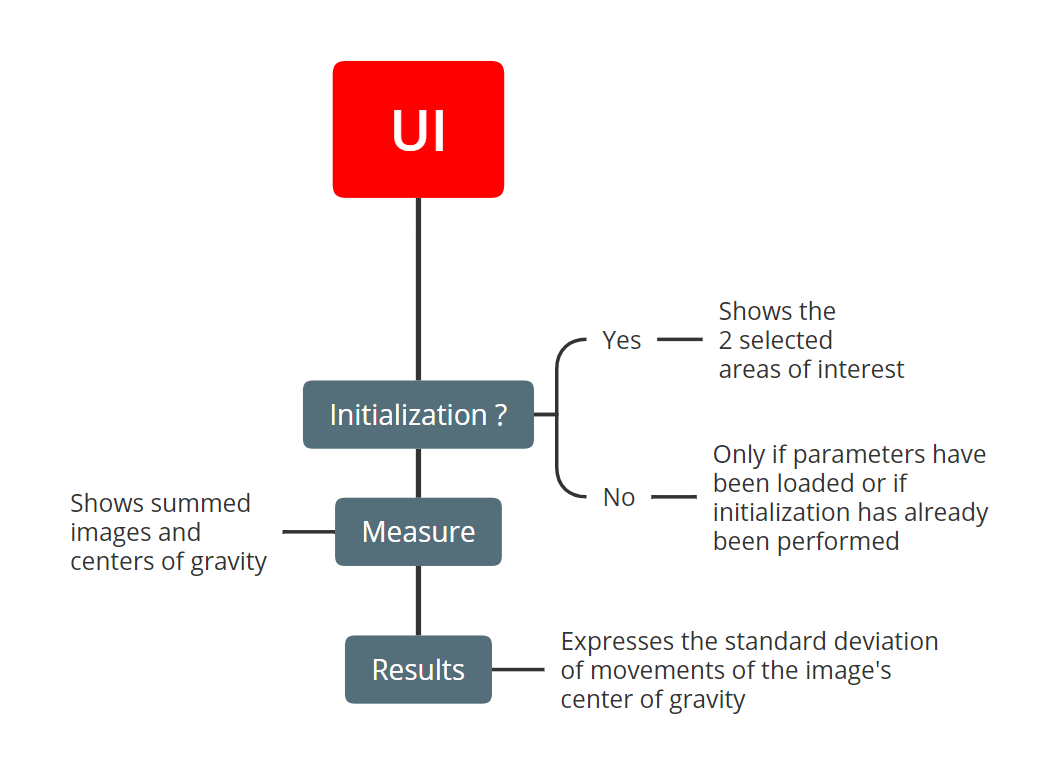
\includegraphics[scale=0.85]{assets/figures/Software/General.png}
    \caption{Software principle as seen by the user}
    \label{fig:Soft_General}
\end{figure}
Figure \ref{fig:Soft_General} shows the application's general operating principle. This application may be updated and changes
are to be expected after the first use in real conditions. It would also be interesting to work with potential future users
to optimize it for their needs.
\newpage
\subsection{Initialization}
The initialization program is essential for the measurement to run smoothly. It is also used to optimize the working
time of the measurement program by cropping only the necessary areas of the image. The basic principle of this program
can be seen in figure \ref{fig:Soft_Init}.
\begin{figure}[H]
    \centering
    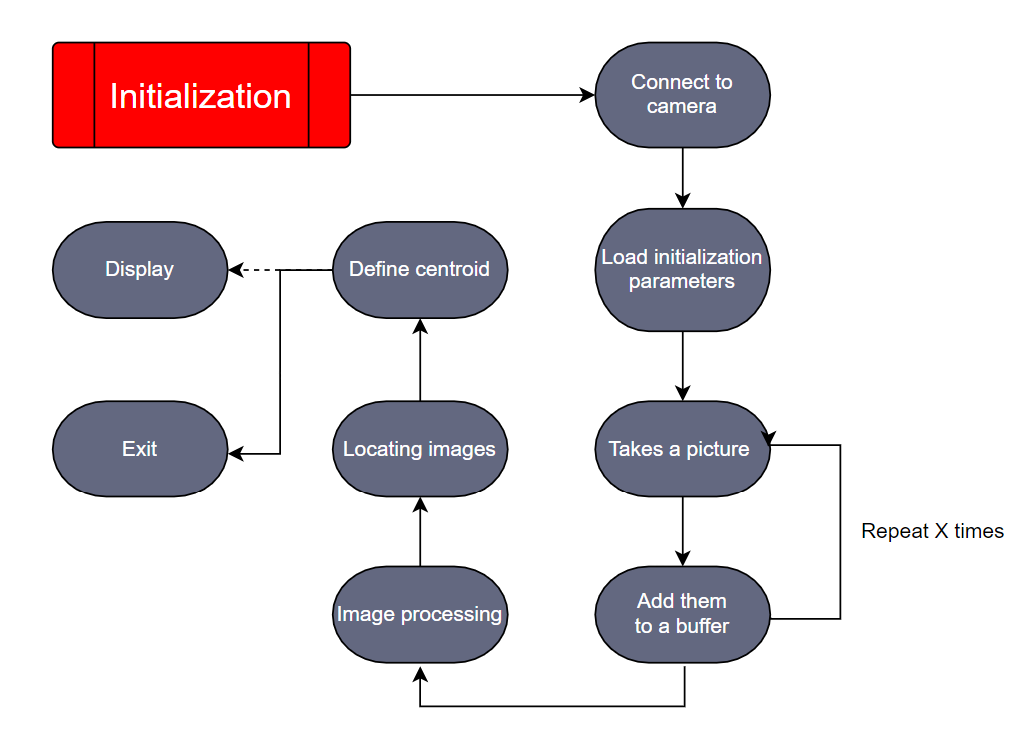
\includegraphics[scale=0.85]{assets/figures/Software/Initialization.png}
    \caption{Block diagram of the initialization function}
    \label{fig:Soft_Init}
\end{figure}
The initialization program performs the following steps :
\begin{enumerate}
    \item Camera connection
    \item Load initialization parameters (e.g. longer exposure time)
    \item Take several images to average out turbulence as far as possible (and as quickly as possible).
    \item Image adjustment (e.g.: clear defaults, increase contrast, etc.)
    \item Location of the 2 focal points of the image
    \item Find the centroid of each area of interest.
    \item Recover and save areas of interest for measurement (Crop image afterwards to reduce processing time)
    \item Display centers of interest if required.
\end{enumerate}
The program principle is the same for all languages. However, for reasons of time, image processing methods and
software accessibility, the program has been written in Python.
\newpage
\subsection{Measurement}
The measurement program is the heart of the system. It enables the measurement to be carried out and the results to be
processed into user-friendly values.The software principle is shown on the block diagram in figure \ref{fig:Soft_Meas}.
\begin{figure}[H]
    \centering
    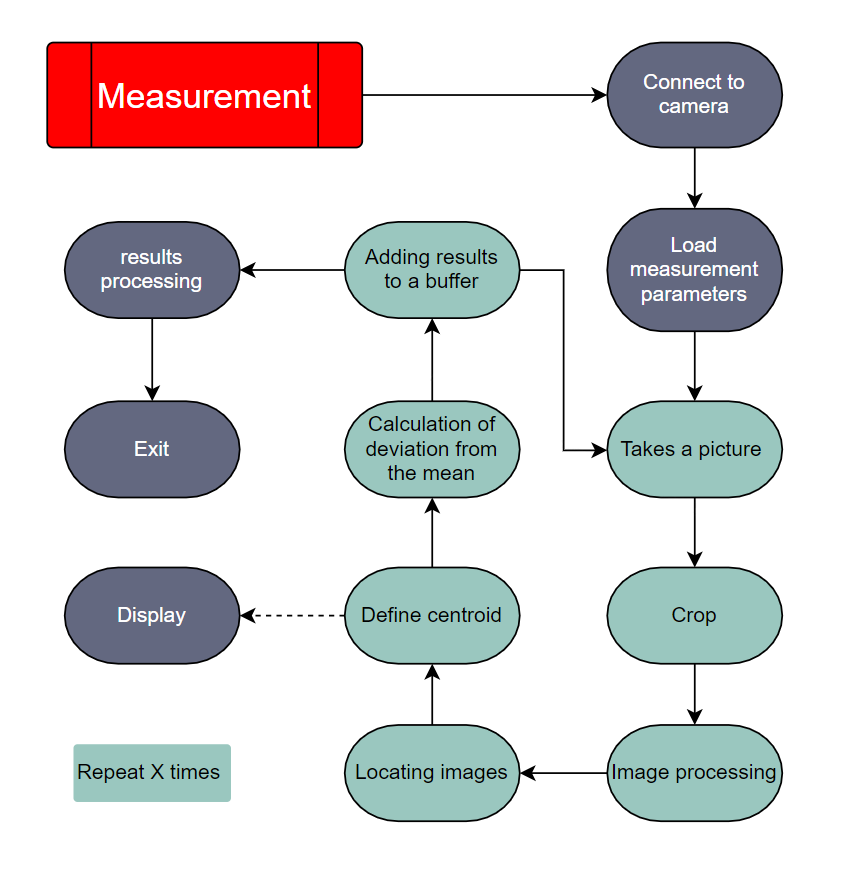
\includegraphics[scale=0.85]{assets/figures/Software/Measurement.png}
    \caption{Block diagram of the measurement function}
    \label{fig:Soft_Meas}
\end{figure}
Cropping the image will considerably reduce process time. The crop ratio will depend on the objects observed.
\bigbreak
The results process simply calculates the standard deviation of the centroid measurements taken.
\begin{equation}
    \sigma = \sqrt{\frac{1}{N}\sum\left(X-X_{init}\right)^2}
\end{equation}
This calculation can be performed for X and Y coordinates and for the total distance calculated using Pythagoras.
However, you'll need to express the standard deviation in arc-seconds using :
\textbf{\textcolor{red}{AJOUTER CALCUL}}
\newline
Once the standard deviation has been calculated, Fried's parameter can be determined by taking the coefficient $r_0$ out of
equation \ref{eq:Opti_Sigma}:
\begin{equation}
    r_0 = 0.1698^{3/5}*\left(\frac{\lambda}{\sigma}\right)^{6/5}*\left(\frac{1}{D}\right)^{1/5}
\end{equation}
\newpage
\subsection{User interface}
To facilitate the use of the system, it was decided to create a user interface.
This window will contain all the elements required to use the \Gls{DIMM}.
\begin{figure}[H]
    \centering
    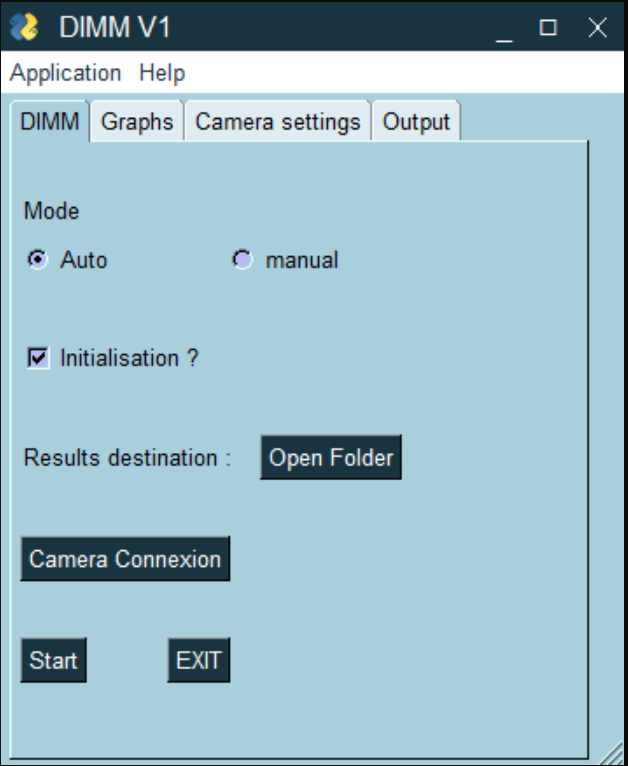
\includegraphics[scale=0.85]{assets/figures/Software/GUI1.png}
    \caption{User interface visualization}
    \label{fig:Soft_GUI}
\end{figure}
The first version of the user interface is shown in Figure \ref{fig:Soft_GUI}.
This application contains all options available for \Gls{DIMM} use :
\begin{itemize}
    \item "\Gls{DIMM}" page : This is the main part of the application. It allows you to select the measurement mode,
          whether the measurement needs to be initialized, the location of the results file and the camera connection test.
    \item "Graphs" page : This page will show the evolution of results over time.
    \item "Camera settings" page : This part of the application performs exactly the same functions as the VIMBA application.
          However, if parameters need to be adjusted in real time, it will be possible to modify them directly on the application.
          You can also use this page to save or load parameter files on your computer.
    \item "Output" page : This page will ensure that the image you have taken is the one you expected.
          The first measurement will be displayed in this section so that you can debug the system in the event of an error,
          or check the measurement if the result looks suspicious.
    \item The "help" section contains instructions for setting up the system.
\end{itemize}